\chapter{粘性流体动力学}

\intro{大自然只认识真实的流体。理想流体是我们发明的第一个近似，而粘性流体是第二个，也是最接近真实的那一个。}

\section{粘性应力的本构关系}

流体区别于固体的本质特征在于其在剪切力作用下能够连续变形。当流体各部分之间以不同速度运动时，粘性摩擦力便会出现，使运动较快的流体层减速，运动较慢的流体层加速。这种动量输运的微观机制是分子热运动导致的动量交换。

\begin{mydefinition}{牛顿粘性定律}
最简单的一维剪切流动中，粘性切应力与速度梯度成正比：
\begin{myformula}
    \tau_{yx} = \mu \frac{du}{dy}
\end{myformula}
其中 $\tau_{yx}$ 为作用于 $y$ 法向平面上、沿 $x$ 方向的切应力，$\mu$ 为动力粘性系数，单位为 $\mathrm{Pa\cdot s}$。运动粘性系数定义为 $\nu = \mu/\rho$，单位为 $\mathrm{m^2/s}$。
\end{mydefinition}

满足牛顿粘性定律的流体称为牛顿流体。水、空气、甘油等常见流体在通常条件下均表现出良好的牛顿流体行为。然而，许多工业流体（如高分子溶液、血液、油漆、泥浆）呈现非牛顿特性，其粘性系数依赖于剪切率或变形历史。

\begin{mydefinition}{非牛顿流体的分类}
常见的非牛顿流体模型包括：
\begin{itemize}
    \item \textbf{幂律流体}：$\tau = K\dot{\gamma}^{n}$，其中 $n<1$ 为假塑性（剪切变稀），$n>1$ 为胀流性（剪切增稠）
    \item \textbf{Bingham塑性体}：$\tau = \tau_y + \mu_p\dot{\gamma}$，存在屈服应力 $\tau_y$
    \item \textbf{粘弹性流体}：同时具有粘性和弹性，如Maxwell模型、Oldroyd-B模型
\end{itemize}
\end{mydefinition}

\subsection{广义牛顿流体的应力张量}

三维情形下，流体的应力状态需用应力张量 $\sigma_{ij}$ 描述。根据Cauchy应力原理，$\sigma_{ij}$ 表示作用于 $i$ 法向平面上、沿 $j$ 方向的应力分量。应力张量可分解为各向同性部分（压力）与偏应力部分（粘性应力）：

\begin{myformula}
    \sigma_{ij} = -p\delta_{ij} + \tau_{ij}
\end{myformula}

其中 $p$ 为热力学压力，$\delta_{ij}$ 为Kronecker符号，$\tau_{ij}$ 为粘性应力张量（偏应力张量），满足 $\tau_{ii}=0$。

对于牛顿流体，Stokes在1845年提出了广义牛顿粘性定律，建立了粘性应力与变形率张量之间最一般的线性各向同性关系：

\begin{myformula}
    \tau_{ij} = 2\mu e_{ij} + \lambda e_{kk}\delta_{ij}
\end{myformula}

其中 $e_{ij} = \frac{1}{2}\left(\frac{\partial u_i}{\partial x_j} + \frac{\partial u_j}{\partial x_i}\right)$ 为变形率张量（应变率张量），$e_{kk} = \nabla\cdot\mathbf{u}$ 为体积膨胀率。$\mu$ 为第一粘性系数（剪切粘性系数），$\lambda$ 为第二粘性系数（体积粘性系数）。

根据Stokes假设，体积粘性系数与剪切粘性系数的关系为 $\lambda = -\frac{2}{3}\mu$。此假设的物理依据是：各向同性膨胀不应引起粘性应力。在此假设下，粘性应力张量简化为：

\begin{myformula}
    \tau_{ij} = 2\mu\left(e_{ij} - \frac{1}{3}e_{kk}\delta_{ij}\right)
\end{myformula}

或等价地写为 $\tau_{ij} = \mu\left(\frac{\partial u_i}{\partial x_j} + \frac{\partial u_j}{\partial x_i} - \frac{2}{3}\frac{\partial u_k}{\partial x_k}\delta_{ij}\right)$。

对于不可压缩流体（$\nabla\cdot\mathbf{u}=0$），表达式进一步简化为 $\tau_{ij} = \mu\left(\frac{\partial u_i}{\partial x_j} + \frac{\partial u_j}{\partial x_i}\right)$。

\begin{figure}[H]
\centering
\begin{tikzpicture}[scale=1.2]
    \definecolor{myfluid}{RGB}{100,149,237}
    \definecolor{myarrow}{RGB}{178,34,34}
    \definecolor{myplate}{RGB}{105,105,105}
    \definecolor{mytop}{RGB}{192,192,192}
    
    \fill[mytop] (0,3) rectangle (5,3.3);
    \fill[myplate] (0,-0.3) rectangle (5,0);
    
    \fill[myfluid!20] (0,0) rectangle (5,3);
    
    \foreach \y in {0.3,0.9,1.5,2.1,2.7} {
        \draw[->, myarrow, line width=1.2pt] (1,\y) -- (1+0.8*\y/3,\y);
        \draw[->, myarrow, line width=1.0pt] (2.5,\y) -- (2.5+0.8*\y/3,\y);
        \draw[->, myarrow, line width=0.8pt] (4,\y) -- (4+0.8*\y/3,\y);
    }
    
    \draw[<->] (0.5,0) -- (0.5,3) node[midway,left] {$h$};
    \node at (0.4,3.3) {$U$};
    \node at (-0.2,1.5) {$y$};
    \node at (3,0.15) {$x$};
    
    \draw[->, line width=1pt] (5.5,1.5) -- (6.8,1.5);
    \node at (5.7,2.3) {Couette};
    \node at (5.7,2.0) {流动};
\end{tikzpicture}
\caption{Couette流动示意图：上平板以速度 $U$ 运动，带动流体层间产生线性速度剖面}
\label{fig:couette-sketch}
\end{figure}

\begin{myTheorem}{应力张量的对称性}
在不存在体力偶的条件下，应力张量是对称的：$\sigma_{ij} = \sigma_{ji}$。这一性质由角动量守恒保证，对于牛顿流体自动满足，因为变形率张量本身是对称的。
\end{myTheorem}

\begin{remark}
对于空气等气体，在标准条件下 $\mu \approx 1.8\times 10^{-5}\;\mathrm{Pa\cdot s}$；对于水，$\mu \approx 1.0\times 10^{-3}\;\mathrm{Pa\cdot s}$。温度对粘性系数有显著影响：气体粘度随温度升高而增加（$\mu \propto \sqrt{T}$），液体粘度随温度升高而降低。
\end{remark}

\section{Navier-Stokes方程的推导}

Navier-Stokes方程是流体力学的基本控制方程，描述了粘性流体运动的动量守恒。其推导基于三个基本物理原理：质量守恒（连续性方程）、动量守恒（牛顿第二定律）以及牛顿流体的本构关系。

\subsection{连续性方程}

连续性方程是质量守恒的微分表述。考虑一个固定的控制体，单位时间内控制体内质量的变化等于通过控制面流入流出的净质量通量：

\begin{myformula}
    \frac{\partial\rho}{\partial t} + \frac{\partial(\rho u_j)}{\partial x_j} = 0
\end{myformula}

或写为物质导数形式：

\begin{myformula}
    \frac{D\rho}{Dt} + \rho\frac{\partial u_j}{\partial x_j} = 0
\end{myformula}

其中物质导数 $\frac{D}{Dt} = \frac{\partial}{\partial t} + u_j\frac{\partial}{\partial x_j}$ 表示跟随流体微团运动时的变化率。

对于不可压缩流体，密度沿质点轨迹保持不变（$\frac{D\rho}{Dt}=0$），但流场中各处密度可以不同（如分层流）。若密度在整个流场中为常数（均质不可压流），则连续性方程简化为：

\begin{myformula}
    \frac{\partial u_i}{\partial x_i} = \nabla\cdot\mathbf{u} = 0
\end{myformula}

\subsection{动量方程（Cauchy运动方程）}

将牛顿第二定律应用于流体微团，得到Cauchy运动方程：

\begin{myformula}
    \rho\frac{D u_i}{D t} = \frac{\partial \sigma_{ij}}{\partial x_j} + \rho g_i
\end{myformula}

将应力张量分解为 $\sigma_{ij} = -p\delta_{ij} + \tau_{ij}$，得到：

\begin{myformula}
    \rho\frac{D u_i}{D t} = -\frac{\partial p}{\partial x_i} + \frac{\partial \tau_{ij}}{\partial x_j} + \rho g_i
\end{myformula}

\subsection{本构关系代入——完整NS方程}

将牛顿流体的本构关系 $\tau_{ij} = \mu\left(\frac{\partial u_i}{\partial x_j} + \frac{\partial u_j}{\partial x_i}\right) + \lambda\frac{\partial u_k}{\partial x_k}\delta_{ij}$ 代入Cauchy运动方程。首先计算粘性力项：

\begin{myformula}
    \frac{\partial\tau_{ij}}{\partial x_j} = \mu\frac{\partial^2 u_i}{\partial x_j\partial x_j} + (\mu+\lambda)\frac{\partial}{\partial x_i}\left(\frac{\partial u_k}{\partial x_k}\right)
\end{myformula}

这里假设了粘性系数 $\mu$ 和 $\lambda$ 为常数。代入后得到可压缩牛顿流体的Navier-Stokes方程：

\begin{myformula}
    \rho\frac{D u_i}{D t} = -\frac{\partial p}{\partial x_i} + \mu\frac{\partial^2 u_i}{\partial x_j\partial x_j} + (\mu+\lambda)\frac{\partial}{\partial x_i}\left(\frac{\partial u_k}{\partial x_k}\right) + \rho g_i
\end{myformula}

这是最一般的可压缩牛顿流体控制方程。方程右端各项的物理意义依次为：压力梯度力、剪切粘性力（粘性扩散）、体积粘性力、体积力。

\begin{myTheorem}{Navier-Stokes方程的张量形式}
完整的可压缩Navier-Stokes方程用物质导数表示为：
\begin{myformula}
    \rho\frac{D u_i}{D t} = -\frac{\partial p}{\partial x_i} + \frac{\partial}{\partial x_j}\left[\mu\left(\frac{\partial u_i}{\partial x_j} + \frac{\partial u_j}{\partial x_i}\right) + \lambda\frac{\partial u_k}{\partial x_k}\delta_{ij}\right] + \rho g_i
\end{myformula}
\end{myTheorem}

\section{不可压缩Navier-Stokes方程}

对于大多数工程问题，流动速度远小于声速，流体可视为不可压缩的。在不可压缩假设下（$\frac{\partial u_k}{\partial x_k}=0$），Navier-Stokes方程大幅简化。

\subsection{基本形式}

不可压缩Navier-Stokes方程的矢量形式是最常使用的表述：

\begin{myformula}
    \frac{\partial\mathbf{u}}{\partial t} + \mathbf{u}\cdot\nabla\mathbf{u} = -\frac{1}{\rho}\nabla p + \nu\nabla^{2}\mathbf{u} + \mathbf{g}
\end{myformula}

其中 $\nu = \mu/\rho$ 为运动粘性系数。配合不可压缩连续性方程 $\nabla\cdot\mathbf{u}=0$，构成封闭方程组。展开为分量形式：

\begin{myformula}
    \frac{\partial u_i}{\partial t} + u_j\frac{\partial u_i}{\partial x_j} = -\frac{1}{\rho}\frac{\partial p}{\partial x_i} + \nu\frac{\partial^{2} u_i}{\partial x_j\partial x_j} + g_i
\end{myformula}

\begin{remark}
不可压缩假设将未知量从未知量减少到四个（三个速度分量 + 压力），方程也是四个（三个动量方程 + 连续性方程），构成适定的初边值问题。压力扮演了"Lagrange乘子"的角色，强制速度场满足无散条件。
\end{remark}

\begin{mydefinition}{NS方程中各项的物理意义}
惯性项 $\mathbf{u}\cdot\nabla\mathbf{u}$（非线性对流项）表示速度场对流自身产生的动量输运，是导致流动复杂性的根源。粘性项 $\nu\nabla^{2}\mathbf{u}$ 表示分子扩散引起的动量输运，起耗散和平滑作用。压力梯度项 $-\frac{1}{\rho}\nabla p$ 驱动流动并维持不可压缩性约束。
\end{mydefinition}

\subsection{压力Poisson方程}

对动量方程取散度，利用不可压缩条件，可导出压力的Poisson方程：

\begin{myformula}
    \nabla^{2} p = -\rho\frac{\partial u_i}{\partial x_j}\frac{\partial u_j}{\partial x_i} = -\rho\nabla\cdot(\mathbf{u}\cdot\nabla\mathbf{u})
\end{myformula}

这表明压力场由速度场的瞬时分布决定，而非独立的热力学变量。这一性质对数值求解有重要意义：求解NS方程时通常采用投影法（分数步法），先求解不含压力梯度的动量方程，再利用Poisson方程修正压力以强制满足无散条件。

\subsection{能量方程}

对于不可压缩流体，能量方程（温度方程）与动量方程解耦，可在速度场求得后单独求解：

\begin{myformula}
    \rho c_p\frac{D T}{D t} = k\nabla^{2} T + \Phi
\end{myformula}

其中 $\Phi = 2\mu e_{ij}e_{ij}$ 为粘性耗散函数，表示机械能不可逆地转化为内能的速率。$c_p$ 为定压比热容，$k$ 为导热系数。

\begin{mycode}{Python：二维方腔驱动流的数值求解}
\begin{lstlisting}[language=Python]
import numpy as np
import matplotlib.pyplot as plt

def solve_cavity_flow(nx, ny, Re, tol=1e-6, max_iter=5000):
    dx, dy = 1.0/(nx-1), 1.0/(ny-1)
    u = np.zeros((ny, nx))
    v = np.zeros((ny, nx))
    p = np.zeros((ny, nx))
    
    u[-1, :] = 1.0
    
    for it in range(max_iter):
        un, vn = u.copy(), v.copy()
        
        u[1:-1, 1:-1] = (un[1:-1, 1:-1]
            - un[1:-1, 1:-1] * dx/(2*dx) * (un[2:, 1:-1] - un[:-2, 1:-1])
            - vn[1:-1, 1:-1] * dy/(2*dy) * (un[1:-1, 2:] - un[1:-1, :-2])
            + dx**2/Re * ((un[2:, 1:-1] - 2*un[1:-1, 1:-1] + un[:-2, 1:-1])/dx**2
            + (un[1:-1, 2:] - 2*un[1:-1, 1:-1] + un[1:-1, :-2])/dy**2))
        
        v[1:-1, 1:-1] = (vn[1:-1, 1:-1]
            - un[1:-1, 1:-1] * dx/(2*dx) * (vn[2:, 1:-1] - vn[:-2, 1:-1])
            - vn[1:-1, 1:-1] * dy/(2*dy) * (vn[1:-1, 2:] - vn[1:-1, :-2])
            + dx**2/Re * ((vn[2:, 1:-1] - 2*vn[1:-1, 1:-1] + vn[:-2, 1:-1])/dx**2
            + (vn[1:-1, 2:] - 2*vn[1:-1, 1:-1] + vn[1:-1, :-2])/dy**2))
        
        u[:, 0] = 0; u[:, -1] = 0; u[0, :] = 0; u[-1, :] = 1.0
        v[:, 0] = 0; v[:, -1] = 0; v[0, :] = 0; v[-1, :] = 0
        
        dudx = (u[1:, :] - u[:-1, :]) / dx
        dvdy = (v[:, 1:] - v[:, :-1]) / dy
        rhs = dudx[:-1, :-1] + dvdy[:-1, :-1]
        
        pn = p.copy()
        p[1:-1, 1:-1] = 0.25 * (pn[2:, 1:-1] + pn[:-2, 1:-1]
            + pn[1:-1, 2:] + pn[1:-1, :-2] - dx**2 * rhs)
        
        p[:, 0] = p[:, 1]; p[:, -1] = p[:, -2]
        p[0, :] = p[1, :]; p[-1, :] = p[-2, :]
        
        u[1:-1, 1:-1] -= dx/(2*dx) * (p[2:, 1:-1] - p[:-2, 1:-1])
        v[1:-1, 1:-1] -= dx/(2*dy) * (p[1:-1, 2:] - p[1:-1, :-2])
        
        if np.max(np.abs(u - un)) < tol and np.max(np.abs(v - vn)) < tol:
            print(f"Converged at iteration {it}")
            break
    return u, v, p

u, v, p = solve_cavity_flow(41, 41, Re=100)

fig, ax = plt.subplots(1, 2, figsize=(12, 5))
X, Y = np.meshgrid(np.linspace(0, 1, 41), np.linspace(0, 1, 41))
ax[0].streamplot(X, Y, u, v, density=1.5, color='k')
ax[0].set_title('Streamlines (Re=100)')
ax[0].set_xlabel('x'); ax[0].set_ylabel('y')

ax[1].contourf(X, Y, np.sqrt(u**2 + v**2), levels=20, cmap='hot')
ax[1].set_title('Velocity magnitude')
ax[1].set_xlabel('x'); ax[1].set_ylabel('y')
plt.colorbar(ax[1].collections[0], ax=ax[1])
plt.tight_layout(); plt.show()
\end{lstlisting}
\end{mycode}

\section{Navier-Stokes方程的无量纲化}

物理问题的无量纲化揭示了控制参数的本质，使我们能够识别决定流动状态的少数无量纲数。

\subsection{无量纲化过程}

引入特征尺度：特征长度 $L$、特征速度 $U$、特征时间 $L/U$、特征压力 $\rho U^{2}$（或 $\mu U/L$）。定义无量纲变量（以星号标记）：

\begin{myformula}
    \mathbf{x}^{*} = \frac{\mathbf{x}}{L},\quad \mathbf{u}^{*} = \frac{\mathbf{u}}{U},\quad t^{*} = \frac{t}{L/U},\quad p^{*} = \frac{p}{\rho U^{2}}
\end{myformula}

将上述无量纲变量代入不可压缩NS方程，得到：

\begin{myformula}
    \frac{\partial\mathbf{u}^{*}}{\partial t^{*}} + \mathbf{u}^{*}\cdot\nabla^{*}\mathbf{u}^{*} = -\nabla^{*} p^{*} + \frac{1}{Re}\nabla^{*2}\mathbf{u}^{*} + \frac{1}{Fr^{2}}\frac{\mathbf{g}}{g}
\end{myformula}

\subsection{Reynolds数及其物理意义}

\begin{mydefinition}{Reynolds数}
Reynolds数定义为惯性力与粘性力之比：
\begin{myformula}
    Re = \frac{UL}{\nu} = \frac{\rho U L}{\mu}
\end{myformula}
\end{mydefinition}

Reynolds数是流体力学中最重要的无量纲数。其物理意义可通过对NS方程中各项的量纲分析来理解：

\begin{itemize}
    \item 惯性项：$\mathbf{u}\cdot\nabla\mathbf{u} \sim U^{2}/L$
    \item 粘性项：$\nu\nabla^{2}\mathbf{u} \sim \nu U/L^{2}$
    \item 二者之比：$\frac{U^{2}/L}{\nu U/L^{2}} = \frac{UL}{\nu} = Re$
\end{itemize}

当 $Re \ll 1$ 时，粘性力主导，流动为爬流（creeping flow），惯性项可忽略，NS方程退化为Stokes方程。当 $Re \gg 1$ 时，惯性力主导，远离壁面处粘性效应可忽略（理想流体近似），但壁面附近必须考虑粘性（边界层概念）。

\subsection{其他重要的无量纲数}

\begin{itemize}
    \item \textbf{Froude数}：$Fr = U/\sqrt{gL}$，惯性力与重力之比，决定自由表面流动的特征
    \item \textbf{Mach数}：$Ma = U/c$，特征速度与声速之比，决定可压缩性效应的重要性（$Ma < 0.3$ 时通常可视为不可压缩）
    \item \textbf{Strouhal数}：$St = fL/U$，非定常惯性力与对流惯性力之比，描述非定常流动特性
    \item \textbf{Weber数}：$We = \rho U^{2}L/\sigma$，惯性力与表面张力之比
    \item \textbf{Euler数}：$Eu = \Delta p/(\rho U^{2})$，压力力与惯性力之比
\end{itemize}

\begin{remark}
几何相似的流动若具有相同的Re数和其他相关无量纲数，则流动相似（动力相似性）。这一原理是风洞实验和水洞实验的理论基础。
\end{remark}

\subsection{不同Re数范围的流动特征}

无量纲化后的NS方程 $\frac{\partial\mathbf{u}^{*}}{\partial t^{*}} + \mathbf{u}^{*}\cdot\nabla^{*}\mathbf{u}^{*} = -\nabla^{*}p^{*} + \frac{1}{Re}\nabla^{*2}\mathbf{u}^{*}$ 清楚地表明，对于给定的几何构型和边界条件，流动的唯一控制参数是Reynolds数。不同Re数对应截然不同的流动状态：

\begin{itemize}
    \item $Re \to 0$：爬流，惯性项消失，方程成为Stokes方程（线性）
    \item $Re \sim O(1)$：层流，粘性和惯性同等重要
    \item $Re \sim O(10^{2})$：定常层流，可能出现回流区
    \item $Re \sim O(10^{3})$：非定常层流，涡脱落现象
    \item $Re \sim Re_{c}$：转捩开始，流动失去稳定性
    \item $Re \to \infty$（形式上）：湍流，惯性主导但粘性在最小尺度上不可或缺
\end{itemize}

\section{Navier-Stokes方程的精确解}

尽管NS方程是非线性的偏微分方程组，在某些简化流动条件下仍可求得精确解析解。这些经典解不仅具有理论价值，更是验证数值方法和理解粘性流动基本特征的重要基准。

\subsection{Couette流动}

考虑两无限长平行平板之间的粘性流动。下板静止，上板以恒定速度 $U$ 沿 $x$ 方向平移。假设流动是定常、充分发展的（$\frac{\partial}{\partial x}=0$，$v=w=0$），且无外加压力梯度。NS方程简化为：

\begin{myformula}
    \frac{d^{2}u}{dy^{2}} = 0
\end{myformula}

在边界条件 $u(0)=0$，$u(h)=U$ 下，解为线性速度剖面：

\begin{myformula}
    u(y) = U\frac{y}{h}
\end{myformula}

壁面切应力为常数：$\tau_w = \mu\frac{du}{dy}\big|_{y=0} = \mu\frac{U}{h}$。

\begin{figure}[H]
\centering
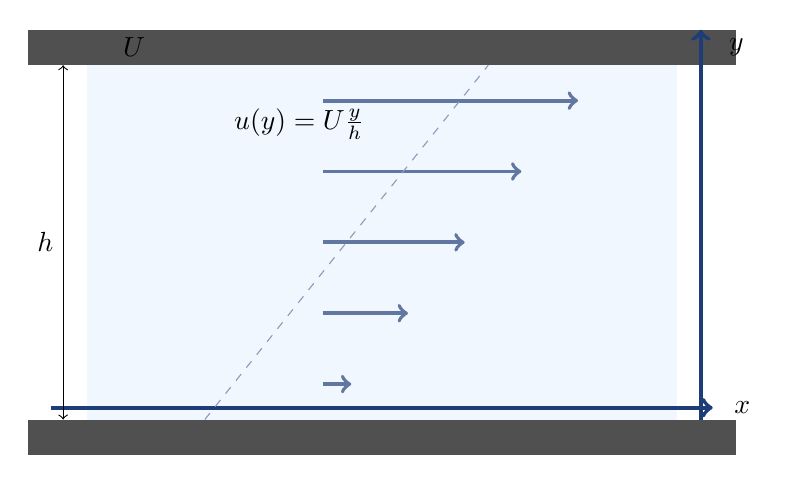
\begin{tikzpicture}[scale=1.5]
    \definecolor{mydark}{RGB}{30,60,120}
    \definecolor{mywall}{RGB}{80,80,80}
    \definecolor{myfluidcol}{RGB}{220,235,255}
    
    \fill[mywall] (-0.5,-0.3) rectangle (5.5,0);
    \fill[mywall] (-0.5,3) rectangle (5.5,3.3);
    \fill[myfluidcol!40] (0,0) rectangle (5,3);
    
    \draw[->, line width=1.5pt, mydark] (5.2,0) -- (5.2,3.3);
    \node at (5.5,3.15) {$y$};
    
    \draw[->, line width=1.5pt, mydark] (-0.3,0.1) -- (5.3,0.1);
    \node at (5.55,0.1) {$x$};
    
    \foreach \y in {0.3,0.9,1.5,2.1,2.7} {
        \pgfmathsetmacro{\ux}{0.8*\y}
        \draw[->, mydark!70, line width=1.4pt] (2,\y) -- (2+\ux,\y);
    }
    
    \draw[dashed, mydark!50] (1,0) -- (1+0.8*3,3);
    \node at (1.8, 2.5) {$u(y)=U\frac{y}{h}$};
    \draw[<->] (-0.2,0) -- (-0.2,3) node[midway,left] {$h$};
    \node at (0.4,3.15) {$U$};
\end{tikzpicture}
\caption{Couette流动的速度剖面：纯剪切驱动下的线性分布}
\label{fig:couette-profile}
\end{figure}

\subsection{Poiseuille流动}

考虑压力梯度驱动下的管道流动。对于二维槽道（平板Poiseuille流），NS方程简化为：

\begin{myformula}
    \frac{dp}{dx} = \mu\frac{d^{2}u}{dy^{2}}
\end{myformula}

其中压力梯度为常数 $G = -dp/dx > 0$。在无滑移边界条件 $u(\pm h)=0$ 下，解为抛物型剖面：

\begin{myformula}
    u(y) = \frac{G}{2\mu}(h^{2} - y^{2})
\end{myformula}

最大速度出现在中心线 $y=0$ 处：$u_{\max} = \frac{Gh^{2}}{2\mu}$。截面平均速度为 $u_{\text{avg}} = \frac{2}{3}u_{\max}$。

对于圆管Poiseuille流（Hagen-Poiseuille流），采用柱坐标，速度剖面为旋转抛物面：

\begin{myformula}
    u(r) = \frac{G}{4\mu}(R^{2} - r^{2})
\end{myformula}

体积流量为著名的Poiseuille公式：$Q = \frac{\pi R^{4}G}{8\mu} = \frac{\pi R^{4}\Delta p}{8\mu L}$。这一关系表明流量与管径的四次方成正比，压降与流量成正比，是层流管道流动的基础。

\begin{figure}[H]
\centering
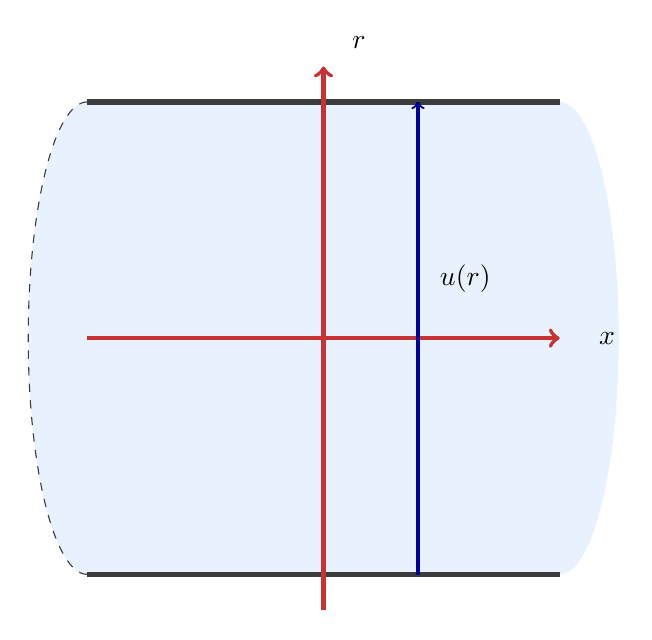
\begin{tikzpicture}[scale=1.5]
    \definecolor{mypipe}{RGB}{60,60,60}
    \definecolor{myfluidcol}{RGB}{180,210,250}
    \definecolor{myprofilecol}{RGB}{200,50,50}
    
    \fill[myfluidcol!30] (-2,0) ellipse (0.5 and 2);
    \fill[myfluidcol!30] (-2,-2) rectangle (2,2);
    \fill[myfluidcol!30] (2,0) ellipse (0.5 and 2);
    
    \draw[mypipe, line width=2pt] (-2,-2) -- (2,-2);
    \draw[mypipe, line width=2pt] (-2,2) -- (2,2);
    \draw[mypipe, dashed] (-2,2) arc(90:270:0.5 and 2);
    
    \draw[->, myprofilecol, line width=1.5pt] (-2,0) -- (2,0);
    \node at (2.4,0) {$x$};
    \draw[->, myprofilecol, line width=1.5pt] (0,-2.3) -- (0,2.3);
    \node at (0.3,2.5) {$r$};
    
    \draw[->, thick, blue!60!black] (0.8,-2) -- (0.8,2);
    \node at (1.2,0.5) {$u(r)$};
    
    \draw[domain=0:1,smooth,variable=\x,blue!60!black,line width=1.8pt]
        plot ({0.8}, {2*(\x^2)});
    \draw[domain=0:1,smooth,variable=\x,blue!60!black,line width=1.8pt]
        plot ({0.8}, {-2*(\x^2)});
\end{tikzpicture}
\caption{圆管Poiseuille流动的旋转抛物面速度剖面}
\label{fig:poiseuille-profile}
\end{figure}

\subsection{Stokes第一问题——突然起动平板}

设半无限大空间 $y \ge 0$ 充满静止粘性流体。$t=0$ 时刻，壁面 $y=0$ 突然以恒定速度 $U$ 沿 $x$ 方向平移。流动由扩散方程描述：

\begin{myformula}
    \frac{\partial u}{\partial t} = \nu\frac{\partial^{2} u}{\partial y^{2}}
\end{myformula}

边界和初始条件：$u(0,t)=U\;(t>0)$，$u(\infty,t)=0$，$u(y,0)=0\;(y>0)$。该问题可通过相似变换求解。引入相似变量 $\eta = y/\sqrt{4\nu t}$，得到自相似解：

\begin{myformula}
    u(y,t) = U\,\mathrm{erfc}\left(\frac{y}{\sqrt{4\nu t}}\right) = U\left[1 - \mathrm{erf}\left(\frac{y}{\sqrt{4\nu t}}\right)\right]
\end{myformula}

其中 $\mathrm{erfc}$ 为余误差函数。壁面切应力随时间衰减：$\tau_w(t) = -\frac{\mu U}{\sqrt{\pi\nu t}} \sim t^{-1/2}$。

\begin{figure}[H]
\centering
\begin{tikzpicture}[scale=3]
    \definecolor{mycurve}{RGB}{20,80,180}
    \definecolor{mywallcol}{RGB}{80,80,80}
    
    \fill[mywallcol] (-0.2,-0.1) rectangle (2.5,0);
    
    \draw[->] (0,0) -- (2.5,0) node[right] {$y$};
    \draw[->] (0,0) -- (0,1.4) node[above] {$u/U$};
    
    \draw[domain=0:2.5,smooth,variable=\y,mycurve,line width=2pt]
        plot ({\y}, {1-erf(\y/0.3)});
    \node at (0.8,0.95) {$t_1$};
    
    \draw[domain=0:2.5,smooth,variable=\y,mycurve!70,line width=2pt]
        plot ({\y}, {1-erf(\y/0.55)});
    \node at (1.4,0.8) {$t_2$};
    
    \draw[domain=0:2.5,smooth,variable=\y,mycurve!50,line width=2pt]
        plot ({\y}, {1-erf(\y/0.8)});
    \node at (2.0,0.6) {$t_3$};
    
    \node at (1.8,0.2) {$t_1<t_2<t_3$};
    \draw[->] (0.4,0.2) -- (0.15,0.05) node[below] {涡量扩散};
    
    \fill[red!40] (0,0) circle (1.2pt);
    \draw[->, red!60] (0.2,0.1) -- (0.1,0.02);
\end{tikzpicture}
\caption{Stokes第一问题：不同时刻的速度剖面。涡量从壁面向外扩散，边界层厚度按 $\sqrt{\nu t}$ 增长}
\label{fig:stokes1}
\end{figure}

\subsection{Stokes第二问题——振荡平板}

壁面以 $U\cos(\omega t)$ 的速度沿 $x$ 方向振荡。经过足够长时间，初始瞬态效应消失，流动达到周期定常状态。NS方程简化为：

\begin{myformula}
    \frac{\partial u}{\partial t} = \nu\frac{\partial^{2} u}{\partial y^{2}}
\end{myformula}

边界条件：$u(0,t)=U\cos(\omega t)$，$u(\infty,t)=0$。设解为 $u(y,t)=\Re\{U e^{i\omega t}f(y)\}$，代入得到 $i\omega f = \nu f''$，其解为：

\begin{myformula}
    u(y,t) = U e^{-y/\delta}\cos\left(\omega t - \frac{y}{\delta}\right)
\end{myformula}

其中 $\delta = \sqrt{2\nu/\omega}$ 为Stokes层厚度（粘性穿透深度）。此解表明振荡在粘性流体中传播时发生指数衰减和相位滞后，$y=\delta$ 处振幅降至壁面的 $1/e$。这一解对理解波浪作用下海底边界层、振荡流中的传热传质等问题具有基础意义。

\section{相似解与量纲分析}

\subsection{Buckingham $\Pi$ 定理}

量纲分析是流体力学中最有力的工具之一。Buckingham $\Pi$ 定理（1914年）陈述：若一个物理问题涉及 $n$ 个物理量，其中包含 $k$ 个基本量纲（在流体力学中通常为质量$[M]$、长度$[L]$、时间$[T]$），则问题可简化为 $n-k$ 个无量纲 $\Pi$ 群之间的关系。

\begin{myalgorithm}{Buckingham $\Pi$ 定理的步骤}
\begin{enumerate}
    \item 列出所有相关的物理量及其量纲
    \item 选择 $k$ 个量纲独立的基本物理量（重复变量）
    \item 将每个剩余物理量与基本物理量组合形成无量纲 $\Pi$ 群
    \item 验证每个 $\Pi$ 群的无量纲性
    \item 最终关系：$\Pi_1 = f(\Pi_2, \Pi_3, \ldots, \Pi_{n-k})$
\end{enumerate}
\end{myalgorithm}

\begin{example}
考虑圆管流动中的压降问题。相关物理量：压降 $\Delta p/L$、管径 $D$、平均速度 $V$、密度 $\rho$、粘度 $\mu$、粗糙度 $\varepsilon$。共有 $n=6$ 个量，含 $k=3$ 个基本量纲。选择 $\rho$、$V$、$D$ 为基本量，导出三个 $\Pi$ 群：

\begin{myformula}
    \Pi_1 = \frac{\Delta p/L}{\rho V^{2}/D} = f_D,\quad \Pi_2 = \frac{\rho V D}{\mu} = Re,\quad \Pi_3 = \frac{\varepsilon}{D}
\end{myformula}

最终得到摩擦因子关系 $f_D = f(Re, \varepsilon/D)$，这就是Moody图的理论基础。
\end{example}

\subsection{自相似解}

自相似解是NS方程的一类特殊解，其速度剖面在不同的空间位置（或时刻）可以通过适当的缩放变换完全重合。数学上，若存在相似变量 $\eta = \eta(x,y)$（或 $\eta = \eta(y,t)$）使得 $u/U = f(\eta)$，则称解为自相似的。

三类经典的流体力学相似解：
\begin{itemize}
    \item \textbf{Stokes第一问题}：$\eta = y/\sqrt{4\nu t}$，前面已讨论
    \item \textbf{Blasius边界层}：$\eta = y\sqrt{U/(\nu x)}$，将在第七章详述
    \item \textbf{平面射流/尾迹}：远场自相似衰减剖面
\end{itemize}

寻找自相似解的通用方法涉及群论（Lie对称性分析）。对偏微分方程施加伸缩变换群，寻找使方程不变的变换，进而确定相似变量的形式。

\subsection{NS方程的量纲分析要点}

从无量纲NS方程可以看出，粘性项乘以 $1/Re$。当 $Re \gg 1$ 时，粘性项在大部分区域可忽略，流动近似为无粘的。但这是奇异摄动问题：无论 $Re$ 多大，壁面处必须满足无滑移条件，粘性始终重要。这一观察直接导向Prandtl的边界层理论。

\section{Navier-Stokes方程的数学性质}

\subsection{非线性性质}

NS方程的数学难点全部源于对流项的非线性。这一非线性有若干关键后果：

\begin{enumerate}
    \item \textbf{非唯一性}：同一边界条件下可能存在多个定常解（分岔现象）
    \item \textbf{解的奇异性}：三维情形下可能出现有限时间奇异性
    \item \textbf{混沌与湍流}：高Re下对初值极度敏感的混沌行为
    \item \textbf{能量级串}：非线性相互作用将能量从大尺度传递到小尺度
\end{enumerate}

\subsection{能量守恒与耗散}

对于不可压缩NS方程，在无滑移边界条件和无体力的情况下，总动能满足：

\begin{myformula}
    \frac{d}{dt}\int_{V} \frac{1}{2}|\mathbf{u}|^{2}\,dV = -\nu\int_{V} |\nabla\mathbf{u}|^{2}\,dV \le 0
\end{myformula}

这意味着总动能随时间衰减，衰减率正比于粘性系数和速度梯度的平方（即拟涡能，enstrophy）。粘性作为唯一的耗散机制不断消耗能量，在定常湍流中由外力做功补充。

\subsection{Helmholtz分解与投影算子}

任一充分光滑的矢量场可唯一分解为无散部分与无旋部分（Hodge分解）：

\begin{myformula}
    \mathbf{u} = \mathbf{u}_{d} + \nabla\phi,\quad \nabla\cdot\mathbf{u}_{d} = 0
\end{myformula}

将Leary投影算子 $\mathcal{P}$（投影到无散子空间）应用于NS方程，可消去压力梯度项：

\begin{myformula}
    \frac{\partial\mathbf{u}}{\partial t} = \mathcal{P}\left[-\mathbf{u}\cdot\nabla\mathbf{u} + \nu\nabla^{2}\mathbf{u}\right]
\end{myformula}

这一抽象形式在泛函分析框架下对研究NS方程的数学性质非常有用。

\subsection{存在性与光滑性——千禧年问题}

三维不可压缩NS方程的解的存在性与光滑性是Clay数学研究所七个千禧年大奖问题之一。问题的精确表述为：给定光滑的初始速度场（满足周期性边界条件和零散度条件），证明或否定三维不可压缩NS方程存在 $\R^{3}\times[0,\infty)$ 上的光滑解。

这一问题的困难在于：非线性项的能量传递机制可能导致速度梯度 $\|\nabla\mathbf{u}\|$ 在有限时间内趋于无穷（blow-up）。二维情形下，由于涡量守恒的额外约束，全局光滑解的存在性已被证明（Ladyzhenskaya, 1969）。但在三维情形下，目前只能证明弱解（Leary-Hopf解）的全局存在性，其光滑性和唯一性仍未完全解决。

\begin{remark}
Ladyzhenskaya在1969年证明了二维NS方程全局光滑解的存在唯一性。三维情形下，若解在有限时间内发生奇异性，则涡量 $\|\boldsymbol{\omega}\|_{\infty}$ 必须发散，且某些Sobolev范数（如 $H^{1/2}$）必须趋于无穷。这些必要条件为数值搜索可能奇异性提供了理论指导。
\end{remark}

\subsection{适定性}

NS方程初边值问题的适定性（Hadamard意义下）要求：
\begin{itemize}
    \item 解存在
    \item 解唯一
    \item 解连续依赖于初边值数据（稳定性）
\end{itemize}

对于二维NS方程，适定性已完整建立。对于三维方程，小时间范围内的局部适定性成立，但全局适定性仍是未解决的问题。能量方法（能量不等式）和Galerkin逼近是证明弱解存在性的主要工具。

\section{低Reynolds数流动——Stokes流动}

当Reynolds数极小时（$Re \to 0$），惯性项相对于粘性项可以忽略。NS方程退化为Stokes方程：

\begin{myformula}
    \nabla p = \mu\nabla^{2}\mathbf{u} + \rho\mathbf{g},\quad \nabla\cdot\mathbf{u}=0
\end{myformula}

或消去重力（将重力的影响吸收到修正压力 $\tilde{p}=p-\rho gz$ 中）：

\begin{myformula}
    \mu\nabla^{2}\mathbf{u} = \nabla\tilde{p},\quad \nabla\cdot\mathbf{u}=0
\end{myformula}

\subsection{Stokes方程的基本性质}

Stokes方程是线性的，因此具有叠加原理。同时，Stokes方程对时间反转是对称的（运动学可逆性），这与Navier-Stokes方程形成鲜明对比。流动的可逆性意味着：若边界运动反向，流体质点将沿原路径返回。

Stokes方程的另一重要性质是最小耗散原理：满足不可压缩条件和给定边界速度的所有运动学容许速度场中，Stokes流动的真实速度场使总能量耗散率 $\Phi = 2\mu\int_V e_{ij}e_{ij}dV$ 取最小值。

\begin{myTheorem}{Stokes流动的倒易定理（Lorentz倒易定理）}
设 $(\mathbf{u},\boldsymbol{\sigma})$ 和 $(\mathbf{u}',\boldsymbol{\sigma}')$ 是同一区域内的两个Stokes流动，则：
\begin{myformula}
    \int_{\partial V} \mathbf{u}\cdot(\boldsymbol{\sigma}'\cdot\mathbf{n})\,dS = \int_{\partial V} \mathbf{u}'\cdot(\boldsymbol{\sigma}\cdot\mathbf{n})\,dS
\end{myformula}
倒易定理是Stokes流动中极其有力的工具，可用来计算颗粒所受的力而不必求解完整的流场。
\end{myTheorem}

\subsection{Stokes阻力公式}

半径为 $a$ 的刚性球以速度 $U$ 在无界粘性流体中平移，Stokes（1851年）求得了绕球流动的解析解。采用球坐标 $(r,\theta,\phi)$，球心位于原点，来流沿极轴方向。Stokes流函数为：

\begin{myformula}
    \psi(r,\theta) = \frac{1}{4}U a^{2}\sin^{2}\theta\left(\frac{a}{r} - \frac{3r}{a} + \frac{2r^{2}}{a^{2}}\right)
\end{myformula}

球表面的应力积分给出了著名的Stokes阻力公式：

\begin{myformula}
    F_D = 6\pi\mu a U
\end{myformula}

其中 $2\pi\mu a U$ 来自压力（形体阻力），$4\pi\mu a U$ 来自粘性剪切（摩擦阻力）。无量纲阻力系数为 $C_D = \frac{F_D}{\frac{1}{2}\rho U^{2}\pi a^{2}} = \frac{24}{Re}$（$Re = 2aU/\nu$）。

\begin{example}
直径为 $10\;\mu\mathrm{m}$ 的球形尘埃颗粒在空气中以 $1\;\mathrm{mm/s}$ 的速度沉降。$Re \approx 6.7\times 10^{-4} \ll 1$，属于Stokes流动范畴。Stokes阻力 $F_D \approx 1.7\times 10^{-12}\;\mathrm{N}$，沉降速度由 $F_D = (\rho_p-\rho_f)g\cdot\frac{4}{3}\pi a^{3}$ 确定。
\end{example}

\subsection{Oseen修正}

Stokes阻力公式在远离球体的区域失效，因为该处惯性项不再可忽略（Whitehead悖论）。Oseen（1910年）通过保留线性化的惯性项改进了远场解。Oseen方程为：

\begin{myformula}
    \rho U\frac{\partial\mathbf{u}}{\partial x} = -\nabla p + \mu\nabla^{2}\mathbf{u}
\end{myformula}

Oseen修正的阻力系数为 $C_D = \frac{24}{Re}\left(1 + \frac{3}{16}Re\right)$，当 $Re$ 较小时改进显著。

\subsection{低Re数流动的应用}

Stokes流动（爬流）在自然界和工程中广泛存在：
\begin{itemize}
    \item 微小颗粒的沉降（气溶胶、泥沙）
    \item 微生物的游动（细菌鞭毛推进、精子运动）
    \item 微流控器件中的流动（芯片实验室）
    \item 多孔介质渗流（地下水、石油开采）
    \item 润滑理论（滑动轴承中的薄层流动）
\end{itemize}

\begin{mycode}{Python：Stokes流动中沉降过程的数值模拟}
\begin{lstlisting}[language=Python]
import numpy as np
import matplotlib.pyplot as plt
from scipy.integrate import solve_ivp

def particle_settling(d_p, rho_p, rho_f, mu, g=9.81):
    a = d_p / 2.0
    m = (4/3) * np.pi * a**3 * rho_p
    buoyant_force = (rho_p - rho_f) * (4/3) * np.pi * a**3 * g
    terminal_velocity_stokes = buoyant_force / (6 * np.pi * mu * a)
    tau = m / (6 * np.pi * mu * a)
    Re_terminal = rho_f * terminal_velocity_stokes * d_p / mu
    
    def ode_system(t, y):
        v = y[0]
        Re = rho_f * abs(v) * d_p / mu
        if Re < 0.1:
            C_D = 24/Re
        elif Re < 1000:
            C_D = (24/Re) * (1 + 0.15 * Re**0.687)
        else:
            C_D = 0.44
        drag = 0.5 * rho_f * C_D * np.pi * a**2 * v * abs(v)
        acc = (buoyant_force - drag) / m
        return [acc]
    
    sol = solve_ivp(ode_system, [0, 10*tau], [0],
        t_eval=np.linspace(0, 10*tau, 200))
    
    fig, axes = plt.subplots(1, 3, figsize=(14, 4))
    axes[0].plot(sol.t/tau, sol.y[0]*100)
    axes[0].set_xlabel('$t/\\tau$')
    axes[0].set_ylabel('Velocity (cm/s)')
    axes[0].axhline(terminal_velocity_stokes*100, color='r',
        linestyle='--', label='Stokes terminal')
    axes[0].legend()
    
    axes[1].plot(sol.t/tau, sol.y[0]/terminal_velocity_stokes)
    axes[1].set_xlabel('$t/\\tau$')
    axes[1].set_ylabel('$v/v_t$ (Stokes)')
    axes[1].set_ylim([0, 1.5])
    
    t_vals = np.logspace(-3, 3, 500)
    Re_vals = t_vals * 0.1
    drag_coeff = 24/Re_vals
    axes[2].loglog(Re_vals, drag_coeff, 'b-', label='Stokes')
    axes[2].set_xlabel('$Re$')
    axes[2].set_ylabel('$C_D$')
    axes[2].legend()
    axes[2].grid(True, alpha=0.3)
    
    plt.tight_layout()
    plt.show()
    
    return terminal_velocity_stokes, Re_terminal

v_t, Re_t = particle_settling(1e-4, 2500, 1.2, 1.8e-5)
print(f"Terminal velocity: {v_t:.4f} m/s, Re = {Re_t:.4e}")
\end{lstlisting}
\end{mycode}

\subsection{润滑理论}

当两个固体表面非常接近（间隙远小于表面特征尺寸），流动可用润滑近似描述。设间隙厚度为 $h(x,y)$，远小于特征长度 $L$（即 $h \ll L$），NS方程简化为：

\begin{myformula}
    \frac{\partial p}{\partial x} = \mu\frac{\partial^{2} u}{\partial z^{2}},\quad
    \frac{\partial p}{\partial y} = \mu\frac{\partial^{2} v}{\partial z^{2}},\quad
    \frac{\partial p}{\partial z} \approx 0
\end{myformula}

积分并利用质量守恒导出经典的Reynolds润滑方程：

\begin{myformula}
    \frac{\partial}{\partial x}\left(h^{3}\frac{\partial p}{\partial x}\right) + \frac{\partial}{\partial y}\left(h^{3}\frac{\partial p}{\partial y}\right) = 6\mu U\frac{\partial h}{\partial x}
\end{myformula}

这一方程是几乎所有滑动轴承设计的理论基础。它能产生极大的压力以支撑载荷，解释了为什么润滑剂能防止固体接触。

\subsection{Hele-Shaw流动}

Hele-Shaw（1898年）发现，粘性流体在两块非常接近的平行平板之间的流动是势流（理想流动）的粘性模拟物。两块平行平板间距为 $b$，流函数满足 $\nabla^{2}\psi = 0$。深度平均速度 $\bar{\mathbf{u}}$ 为无旋场：$\bar{\mathbf{u}} = \nabla\phi$，其中 $\phi = -\frac{b^{2}}{12\mu}p$。这一性质使Hele-Shaw槽成为二维势流可视化的经典实验装置。

\begin{figure}[H]
\centering
\begin{tikzpicture}[scale=1.5]
    \definecolor{myhele}{RGB}{70,130,180}
    \definecolor{myplatecol}{RGB}{100,100,100}
    \definecolor{myobs}{RGB}{60,60,60}
    \definecolor{myline}{RGB}{20,60,130}
    
    \fill[myplatecol!15] (0,0) rectangle (6,3);
    
    \fill[myobs] (3,1.5) ellipse (0.4 and 0.6);
    
    \draw[myline, line width=1pt, domain=0:6, samples=15, variable=\x]
        plot ({\x}, {1.5 + 0.2*sin(2*pi*\x/6 r)});
    \draw[myline, line width=1pt, domain=0:6, samples=15, variable=\x]
        plot ({\x}, {1.5 - 0.2*sin(2*pi*\x/6 r)});
    \draw[myline, line width=1pt, domain=0:6, samples=15, variable=\x]
        plot ({\x}, {1.5 + 0.6*sin(2*pi*\x/6 r)});
    \draw[myline, line width=1pt, domain=0:6, samples=15, variable=\x]
        plot ({\x}, {1.5 - 0.6*sin(2*pi*\x/6 r)});
    \draw[myline, line width=1pt, domain=0:6, samples=15, variable=\x]
        plot ({\x}, {1.5 + 1.0*sin(2*pi*\x/6 r)});
    \draw[myline, line width=1pt, domain=0:6, samples=15, variable=\x]
        plot ({\x}, {1.5 - 1.0*sin(2*pi*\x/6 r)});
    
    \draw[->, line width=1.5pt] (0.5,0.3) -- (5.5,0.3);
    \node at (5.8,0.3) {$x$};
    \draw[->, line width=1.5pt] (0.3,0.5) -- (0.3,2.8);
    \node at (0.3,3.1) {$y$};
    
    \node at (3,-0.3) {Hele-Shaw槽道绕圆柱流动};
\end{tikzpicture}
\caption{Hele-Shaw槽道中绕圆柱的流线：深度平均流动等价于二维势流}
\label{fig:hele-shaw}
\end{figure}

\subsection{多孔介质流动——Darcy定律}

流体在多孔介质中的缓慢流动由Darcy定律（1856年）描述：

\begin{myformula}
    \mathbf{u} = -\frac{k}{\mu}\nabla p
\end{myformula}

其中 $k$ 为渗透率（量纲 $[L^{2}]$），$\mathbf{u}$ 为Darcy速度（表观速度，非孔隙速度）。将Darcy定律与连续性方程结合，得到压力满足的Laplace方程：

\begin{myformula}
    \nabla^{2}p = 0
\end{myformula}

Darcy定律是体积平均的Stokes方程，其有效性的上限为 $Re_k \equiv \frac{\rho U\sqrt{k}}{\mu} \sim O(1)$。在高Re数下，需要Forchheimer修正项 $-\beta\rho|\mathbf{u}|\mathbf{u}$ 来计及惯性效应。

\begin{myTheorem}{Stokes流动与Darcy流动的统一}
将多孔介质抽象为固体基质的集合，在每一孔道内应用Stokes方程，然后进行体积平均，可严格导出Darcy定律。渗透率 $k$ 与微观孔道几何的关系可通过Kozeny-Carman方程估算：
\begin{myformula}
    k = \frac{\phi^{3}}{c S^{2}(1-\phi)^{2}}
\end{myformula}
其中 $\phi$ 为孔隙率，$S$ 为比表面积，$c$ 为Kozeny常数（近似值为5）。
\end{myTheorem}

\section{本章总结}

本章系统阐述了粘性流体动力学的理论基础，从牛顿粘性定律出发，推导了完整的Navier-Stokes方程，并讨论了不可压缩情形下的简化形式。通过无量纲化引入了流动的核心控制参数——Reynolds数。精确解（Couette流、Poiseuille流、Stokes问题）为理解粘性流动提供了重要的理论基准。低Reynolds数极限下的Stokes方程和润滑理论在微尺度流动、多孔介质渗流和生物流体力学中有广泛应用。对NS方程数学性质的讨论揭示了其深刻的理论困难（存在性与光滑性问题），为后续章节（湍流、边界层、涡动力学）奠定了理论基础。
